\newpage
\section{Auswertung}
\label{sec:auswertung}
Die in der Auswertung verwendeten Mittelwerte mehrfach gemessener Größen sind gemäß der Gleichung
%
\begin{equation}
    \bar{x}=\frac{1}{n}\sum_{i=1}^n x_i
    \label{eq:mittelwert}
\end{equation}
%
bestimmt.
Die Standardabweichung des Mittelwertes ergibt sich dabei zu
%
\begin{equation}
    \symup{\Delta}\bar{x}=\sqrt{\frac{1}{n(n-1)}\sum_{i=1}^n\left(x_i-\bar{x}\right)^2}.
    \label{eq:standardabweichung}
\end{equation}
%
Resultiert eine Größe über eine Gleichung aus zwei anderen fehlerbehafteten Größen, so berechnet sich der Gesamtfehler nach der Gaußschen Fehlerfortpflanzung zu
%
\begin{equation}
    \symup{\Delta}f(x_1,x_2,...,x_n)=\sqrt{\left(\frac{\partial f}{\partial x_1}\symup{\Delta}x_1\right)^2+\left(\frac{\partial f}{\partial x_2}\symup{\Delta}x_2\right)^2+ \dotsb +\left(\frac{\partial f}{\partial x_n}\symup{\Delta}x_n\right)^2}.
    \label{eq:fehlerfortpflanzung}
\end{equation}
%
Alle in der Auswertung angegebenen Größen sind stets auf die erste signifikante Stelle des Fehlers gerundet.
Setzt sich eine Größe über mehrere Schritte aus anderen Größen zusammen, so wird erst am Ende gerundet, um Fehler zu vermeiden.
Zur Auswertung wird die Programmiersprache \texttt{python (Version 3.4.1)}
mit den Bibliothekserweiterungen \texttt{numpy}, \texttt{scipy} und \texttt{matplotlib} zur Erstellung der Grafiken und linearen Regressionen verwendet.

%
\subsection{Stabilität des Lasers}
%
Wie in Abschnitt~\ref{sec:theorie} beschrieben, ist der hier verwendete Laser optisch nur dann stabil, wenn das Produkt $g_1\cdot g_2\in[0,1)$ ist. Daher lassen sich Bedingungen an den Abstand der Resonatorspiegel stellen. Im ersten Versuchsteil werden zwei konvexe Spiegel mit dem Krümmungsradius $\SI{140}{\centi\meter}$ verwendet. Über den Zusammenhang
%
\begin{equation}
  L_{1,2}=\frac{r_1+r_2}{2}\pm\sqrt{\frac{(r_1+r_2)^2}{4}-r_1r_2}
\end{equation}
%
folgt somit, dass der Laser für Resonatorlängen zwischen~$\SI{0}{\centi\meter}$ und~$\SI{280}{\centi\meter}$ optisch stabil ist, siehe Abbildung~\ref{fig:opt_stab}.
%
\begin{figure}[h]
  \centering
  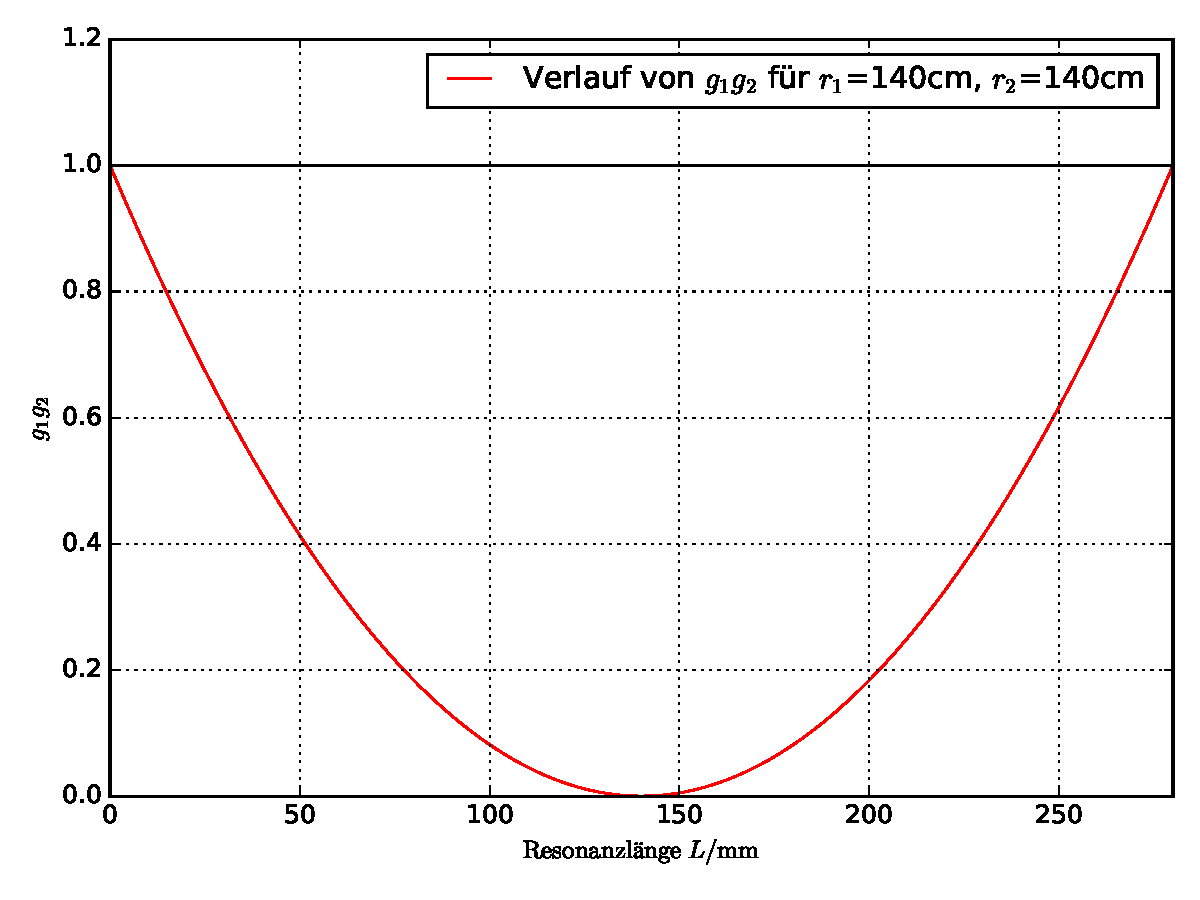
\includegraphics[width=0.8\textwidth]{auswertung/plot_laser_140_140.pdf}
  \caption{Bereich der Resonatorlänge~$L$, in welchem der Laser optisch stabil ist ($g_1\cdot g_2\in[0,1)$).}
  \label{fig:opt_stab}
\end{figure}
%
Da die hier verwedete optische Bank lediglich $\SI{250}{\centi\meter}$ lang ist, kann hier nur überprüft werden, ob die optische Stabilität am
Rande der Bank noch besteht. Dies ist trotz großer Anfälligkeit bei kleinen Abweichungen der Linsen, die allerdings dem experimentellen Aufbau
geschuldet sind, möglich. Eine Messung der Intensität des Laserstrahles in Abhängigkeit der Resonatorlänge ist in Abbildung~\ref{fig:kk}
dargestellt. Es zeigt sich hierbei, dass der Laser bis etwa $\SI{1300}{\milli\meter}$ ununterbrochen mit hoher Leistung funktioniert.
Die Verteilung der Intensitäten zeigt hierbei allerdings auch deutlich das angesprochene Problem: Die Schwankungen der Intensität aufgrund
des experimentellen Aufbaus stellt sich als so stark heraus, dass eine kontinuierliche Messung bis an die Grenze der optischen Bank nicht
durchführbar ist.
%
\begin{figure}[htb]
  \centering
  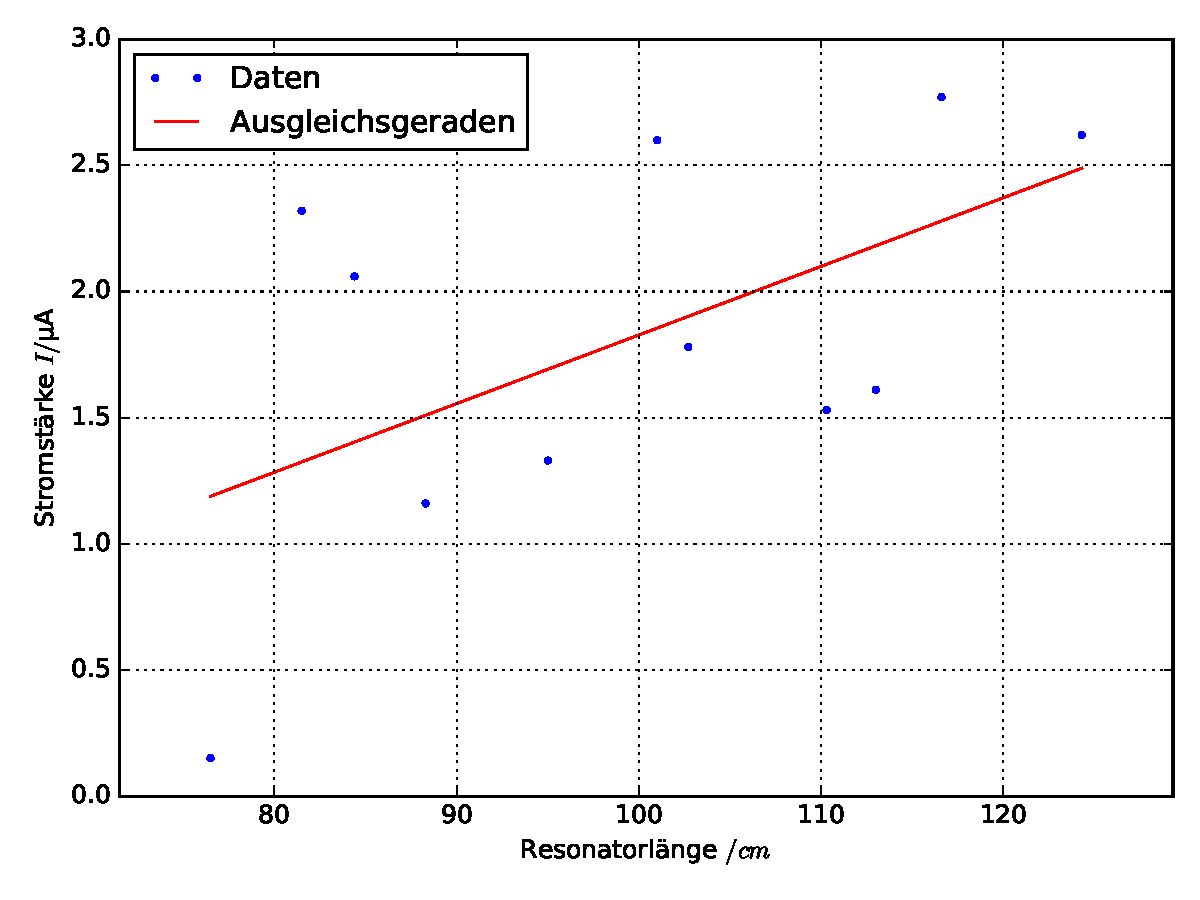
\includegraphics[width=0.8\textwidth]{auswertung/plot_kk.pdf}
  \caption{Darstellung der an der Photodiode gemessenen Stromstärke als Maß für die Intensität des Laserlichtes in Abhängigkeit der Resonatorlänge. Es zeigen sich klar die großen Schwankungen aufgrund der experimentellen Ungenauigkeiten.}
  \label{fig:kk}
\end{figure}
%
\subsection{Vermessung der~$\text{TEM}_{00}$- und der~$\text{TEM}_{10}$-Mode}
%
Im Betrieb bilden sich im Resonator, wie in Abschnitt~\ref{sec:theorie} beschrieben, bestimmte Schwingungsmoden aus. Diese können durch
schrittweise Vermessung untersucht werden. Zunächst wird die~$\text{TEM}_{00}$-Grundmode untersucht. Diese bildet sich im Resonator ohne weitere
Störung durch einen Draht aus. Die Intensität des Lichtes an verschiedenen Punkten einer auf Höhe der Photodiode liegenden Ebene ist in
Tabelle~\ref{tab:tem00} in Form der gemessenen Stromstärke der Photodiode aufgeführt. Die Verteilung dieser Intensität folgt dabei laut Theorie
dem Zusammenhang
%
\begin{equation}
  I(r)=I_0\symup{e}^{\frac{-2(x-x_0)^2}{\omega^2}}.
\end{equation}
%
Mit Hilfe dieser Funktionsvorschrift kann eine Ausgleichsrechnung durchgeführt werden. Das Ergebnis dieser Ausgleichsrechnung, sowie die Messwerte sind in Abbildung~\ref{fig:tem00} dargestellt.
%
\begin{figure}[h]
  \centering
  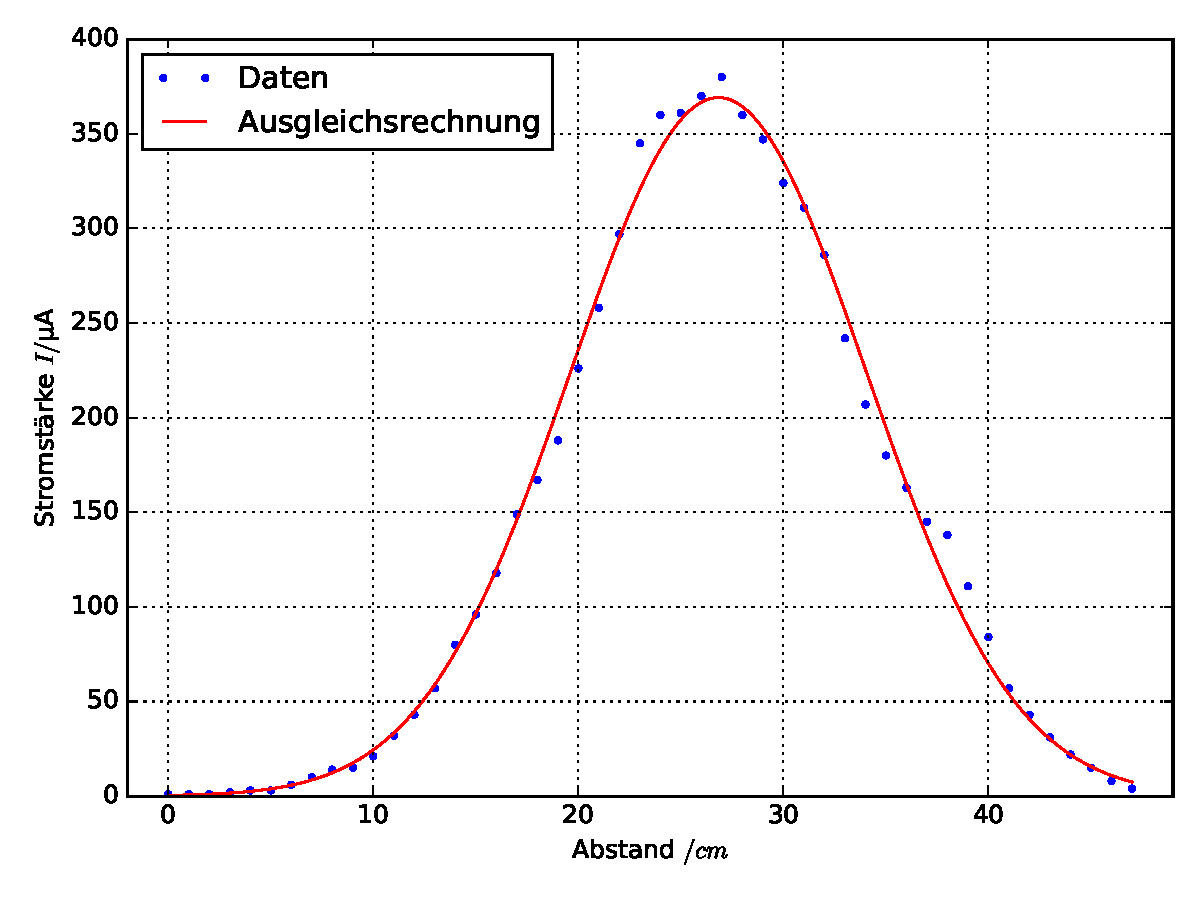
\includegraphics[width=0.8\textwidth]{auswertung/plot_Mode00.pdf}
  \caption{Mit der Photodiode gemessene Stromstärke in Abhängigkeit des Ortes innerhalb des Resonators. Dazu die aus dem theoretischen Modell berechnete Verteilung der Ausgleichsrechnung.}
  \label{fig:tem00}
\end{figure}
%
\begin{table}
  \centering
  \caption{Mit der Photodiode gemessene Stromstärken und Orte innerhalb des Resonators (Nullpunkt willkürlich gewählt).}
  \begin{tabular}{cccc}
    \toprule
    {x [cm]}  & {I [\mu A]} & {x [cm]}  & {I [\mu A]}     \\
		\midrule
	  \SI{0 }{} & \SI{  1}{} & \SI{24}{} & \SI{360}{}\\
    \SI{1 }{} & \SI{  1}{} & \SI{25}{} & \SI{361}{}\\
		\SI{2 }{} & \SI{  1}{} & \SI{26}{} & \SI{370}{}\\
		\SI{3 }{} & \SI{  2}{} & \SI{27}{} & \SI{380}{}\\
		\SI{4 }{} & \SI{  3}{} & \SI{28}{} & \SI{360}{}\\
    \SI{5 }{} & \SI{  3}{} & \SI{29}{} & \SI{347}{}\\
    \SI{6 }{} & \SI{  6}{} & \SI{30}{} & \SI{324}{}\\
    \SI{7 }{} & \SI{ 10}{} & \SI{31}{} & \SI{311}{}\\
    \SI{8 }{} & \SI{ 14}{} & \SI{32}{} & \SI{286}{}\\
    \SI{9 }{} & \SI{ 15}{} & \SI{33}{} & \SI{242}{}\\
    \SI{10}{} & \SI{ 21}{} & \SI{34}{} & \SI{207}{}\\
    \SI{11}{} & \SI{ 32}{} & \SI{35}{} & \SI{180}{}\\
    \SI{12}{} & \SI{ 43}{} & \SI{36}{} & \SI{163}{}\\
    \SI{13}{} & \SI{ 57}{} & \SI{37}{} & \SI{145}{}\\
    \SI{14}{} & \SI{ 80}{} & \SI{38}{} & \SI{138}{}\\
    \SI{15}{} & \SI{ 96}{} & \SI{39}{} & \SI{111}{}\\
    \SI{16}{} & \SI{118}{} & \SI{40}{} & \SI{ 84}{}\\
    \SI{17}{} & \SI{149}{} & \SI{41}{} & \SI{ 57}{}\\
    \SI{18}{} & \SI{167}{} & \SI{42}{} & \SI{ 43}{}\\
    \SI{19}{} & \SI{188}{} & \SI{43}{} & \SI{ 31}{}\\
    \SI{20}{} & \SI{226}{} & \SI{44}{} & \SI{ 22}{}\\
    \SI{21}{} & \SI{258}{} & \SI{45}{} & \SI{ 15}{}\\
    \SI{22}{} & \SI{297}{} & \SI{46}{} & \SI{  8}{}\\
    \SI{23}{} & \SI{345}{} & \SI{47}{} & \SI{  4}{}\\
		\bottomrule
	\end{tabular}
  \label{tab:tem00}
\end{table}
%
Die Ausgleichsrechnung ergibt folgende Parameter:
%
\begin{align*}
  I_0=&\SI{370(3)}{\micro\ampere} \\
  x_0=&\SI{26.83(7)}{\centi\meter} \\
  \omega=&\SI{-10.2(1)}{\centi\meter}
\end{align*}
%
Zur Untersuchung der $\text{TEM}_{10}$-Mode wird diese durch Einbringen eines dünnen Drahtes in den Resonator erzeugt. Anschließend wird wie zuvor die Stromstärke an der Photodiode als Maß für die Intensität des Lichtes für verschiedene Positionen des Drahtes innerhalb des Resonators gemessen. Es ergeben sich die in Tabelle~\ref{tab:tem10} aufgeführten Werte für die Stromstärke.
%
\begin{table}
  \centering
  \caption{Mit der Photodiode gemessene Stromstärken und Orte innerhalb des Resonators (Nullpunkt willkürlich gewählt).}
  \begin{tabular}{cccc}
    \toprule
    {x [cm]}  & {I [\mu A]} & {x [cm]}  & {I [\mu A]}     \\
		\midrule
	  \SI{0 }{} & \SI{ 3.4}{} & \SI{22}{} & \SI{ 0.7}{}\\
    \SI{1 }{} & \SI{ 5.6}{} & \SI{23}{} & \SI{ 2.1}{}\\
		\SI{2 }{} & \SI{ 9.8}{} & \SI{24}{} & \SI{ 4.3}{}\\
		\SI{3 }{} & \SI{13.9}{} & \SI{25}{} & \SI{ 8.0}{}\\
		\SI{4 }{} & \SI{16.5}{} & \SI{26}{} & \SI{12.2}{}\\
    \SI{5 }{} & \SI{23.2}{} & \SI{27}{} & \SI{18.9}{}\\
    \SI{6 }{} & \SI{29.8}{} & \SI{28}{} & \SI{26.0}{}\\
    \SI{7 }{} & \SI{33.2}{} & \SI{29}{} & \SI{36.8}{}\\
    \SI{8 }{} & \SI{36.0}{} & \SI{30}{} & \SI{39.2}{}\\
    \SI{9 }{} & \SI{40.7}{} & \SI{31}{} & \SI{41.2}{}\\
    \SI{10}{} & \SI{43.2}{} & \SI{32}{} & \SI{45.0}{}\\
    \SI{11}{} & \SI{46.7}{} & \SI{33}{} & \SI{43.5}{}\\
    \SI{12}{} & \SI{48.8}{} & \SI{34}{} & \SI{45.6}{}\\
    \SI{13}{} & \SI{45.6}{} & \SI{35}{} & \SI{41.2}{}\\
    \SI{14}{} & \SI{40.9}{} & \SI{36}{} & \SI{36.8}{}\\
    \SI{15}{} & \SI{35.8}{} & \SI{37}{} & \SI{33.5}{}\\
    \SI{16}{} & \SI{24.2}{} & \SI{38}{} & \SI{31.5}{}\\
    \SI{17}{} & \SI{18.8}{} & \SI{39}{} & \SI{24.9}{}\\
    \SI{18}{} & \SI{10.4}{} & \SI{40}{} & \SI{17.7}{}\\
    \SI{19}{} & \SI{ 5.6}{} & \SI{41}{} & \SI{11.4}{}\\
    \SI{20}{} & \SI{ 1.6}{} & \SI{42}{} & \SI{ 8.6}{}\\
    \SI{21}{} & \SI{ 0.2}{} &  & \\
    \bottomrule
	\end{tabular}
  \label{tab:tem10}
\end{table}
%
Die Verteilung dieser Intensität folgt dabei laut Theorie dem Zusammenhang
%
\begin{equation}
  I(r)=I_0\cdot\frac{8(x-x_0)^2}{\omega^2}\cdot\symup{e}^{\frac{-2(x-x_0)^2}{\omega^2}}.
\end{equation}
%
Mit Hilfe dieser Funktionsvorschrift kann eine Ausgleichsrechnung durchgeführt werden. Das Ergebnis dieser Ausgleichsrechnung, sowie die Messwerte sind in Abbildung~\ref{fig:tem10} dargestellt.
%
\begin{figure}[h]
  \centering
  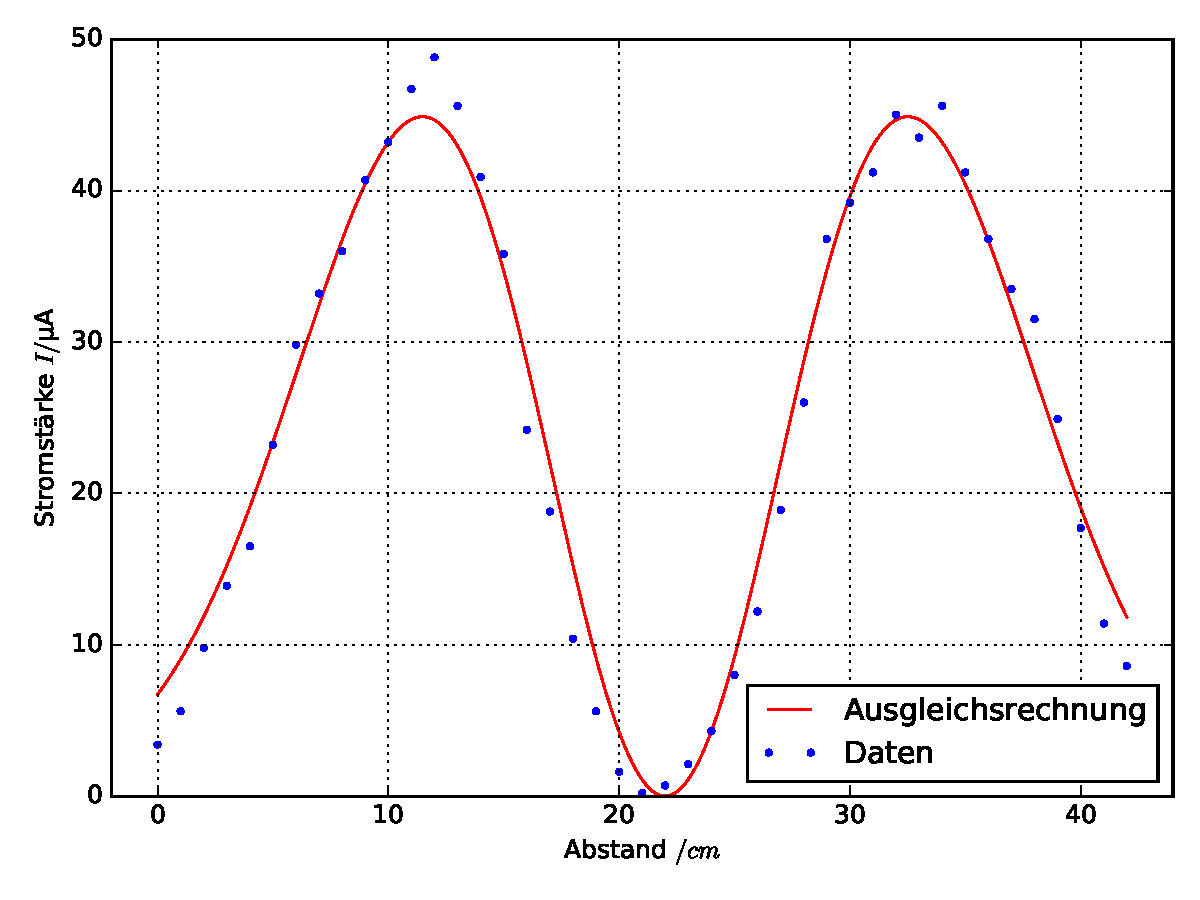
\includegraphics[width=0.8\textwidth]{auswertung/plot_Mode10.pdf}
  \caption{Mit der Photodiode gemessene Stromstärke in Abhängigkeit des Ortes innerhalb des Resonators. Dazu die aus dem theoretischen Modell berechnete Verteilung der Ausgleichsrechnung.}
  \label{fig:tem10}
\end{figure}
%
Die Ausgleichrechnung ergibt für diese Mode folgende Parameter:
%
\begin{align*}
  I_0=&\SI{30.5(4)}{\micro\ampere} \\
  x_0=&\SI{21.99(9)}{\centi\meter} \\
  \omega=&\SI{14.9(1)}{\centi\meter}
\end{align*}
%
Die Intensitätsverteilungen für die beiden betrachteten Moden spiegeln insgesamt ein gutes Bild der stehenden Wellen wider. Die Winkelverteilung
der Messwerte stimmt gut mit der Theorie überein und es lässt sich gut die höhere Ordnung der $\text{TEM}_{10}$-Mode im Vergleich zur $\text{TEM}_{00}$-Mode erkennen.

%
\subsection{Untersuchung der Polarisation des Lasers}
%
Zur Bestimmung der Polarisation des Laserlichtes wird dieses durch einen Polarisationsfilter auf die Photodiode geleitet. Durch Variation
des Polarisationswinkels in~$10°$-Schritten kann das Verhalten der Intensität auf der Photodiode untersucht werden. Die unter den einzelnen
Winkeln gemessenen Photoströme sind in Tabelle~\ref{tab:polarisation} aufgeführt.
%
\begin{table}
  \centering
  \caption{Mit der Photodiode gemessene Stromstärken für verschiedene Winkel des Polarisationsfilters.}
  \begin{tabular}{cccc}
    \toprule
    {$\alpha$ [°]}  & {I [\mu A]} & {$\alpha$ [°]}  & {I [\mu A]}     \\
		\midrule
	  \SI{0 }{}  & \SI{ 53}{} & \SI{190}{} & \SI{147}{}\\
    \SI{10 }{} & \SI{125}{} & \SI{200}{} & \SI{231}{}\\
		\SI{20 }{} & \SI{236}{} & \SI{210}{} & \SI{360}{}\\
		\SI{30 }{} & \SI{355}{} & \SI{220}{} & \SI{503}{}\\
		\SI{40 }{} & \SI{460}{} & \SI{230}{} & \SI{628}{}\\
    \SI{50 }{} & \SI{576}{} & \SI{240}{} & \SI{712}{}\\
    \SI{60 }{} & \SI{618}{} & \SI{250}{} & \SI{699}{}\\
    \SI{70 }{} & \SI{705}{} & \SI{260}{} & \SI{744}{}\\
    \SI{80 }{} & \SI{732}{} & \SI{270}{} & \SI{631}{}\\
    \SI{90 }{} & \SI{559}{} & \SI{280}{} & \SI{564}{}\\
    \SI{100}{} & \SI{507}{} & \SI{290}{} & \SI{386}{}\\
    \SI{110}{} & \SI{413}{} & \SI{300}{} & \SI{288}{}\\
    \SI{120}{} & \SI{291}{} & \SI{310}{} & \SI{184}{}\\
    \SI{130}{} & \SI{177}{} & \SI{320}{} & \SI{ 77}{}\\
    \SI{140}{} & \SI{ 88}{} & \SI{330}{} & \SI{ 21}{}\\
    \SI{150}{} & \SI{ 30}{} & \SI{340}{} & \SI{  1}{}\\
    \SI{160}{} & \SI{  1}{} & \SI{350}{} & \SI{  9}{}\\
    \SI{170}{} & \SI{  9}{} & \SI{360}{} & \SI{ 61}{}\\
    \SI{180}{} & \SI{ 55}{} &  & \\
    \bottomrule
	\end{tabular}
  \label{tab:polarisation}
\end{table}
%
Die Verteilung ist in Abbildung~\ref{fig:polarisation} grafisch dargestellt.
%
\begin{figure}[htb]
  \centering
  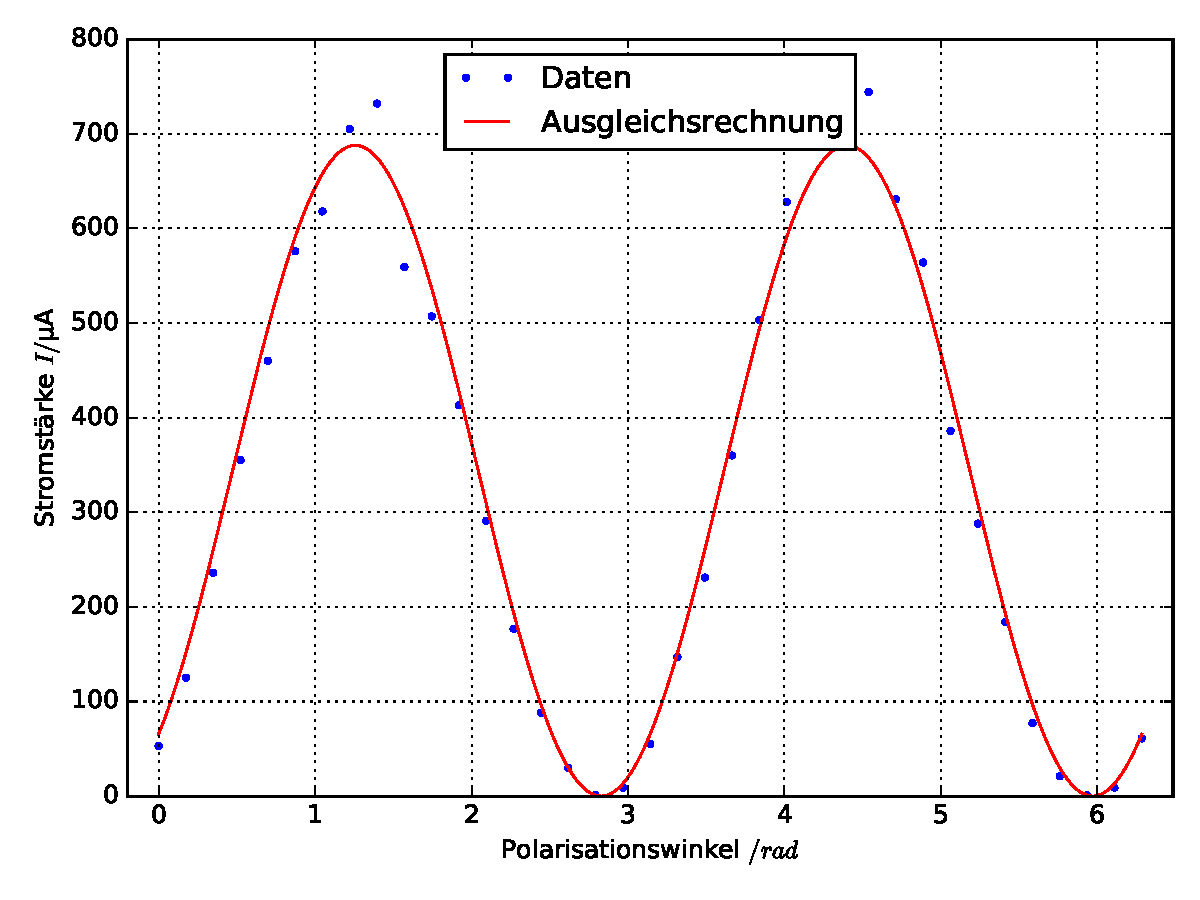
\includegraphics[width=0.8\textwidth]{auswertung/plot_polarisation.pdf}
  \caption{Mit der Photodiode gemessene Stromstärke in Abhängigkeit des Winkels des Polarisationsfilters und Ausgleichsrechnung.}
  \label{fig:polarisation}
\end{figure}
%
Für die Daten zur Polarisation wird eine Ausgleichsrechnung der Form
%
\begin{equation}
  I(x)=I_0\cos(x_0+x)^2
\end{equation}
%
durchgeführt. Die Ergebnisse lauten hierbei:
%
\begin{align*}
  I_0=&\SI{687(8)}{\micro\ampere} \\
  x_0=&\SI{92.99(1)}{}
\end{align*}
%
Es wird deutlich, dass das Laserlicht bei~$\approx 1,2$ rad mit maximaler Intensität den Polarisationsfilter durchläuft.
%
\subsection{Bestimmung der Wellenlänge des Lasers}
%
Zur Bestimmung der Wellenlänge wird das Laserlicht an einem Gitter gebeugt und das so entstehende Interferenzmuster untersucht.
Aus den Abständen~$a$ der~$n$-ten Maxima in diesem Beugungsbild lässt sich zusammen mit der Gitterkonstante~$g$ und dem Abstand~$d$ des
Gitters vom Schirm über den Zusammenhang
%
\begin{equation}
  \lambda=\frac{a}{n\cdot d\cdot g}
\end{equation}
%
die Wellenlänge des Laserlichtes berechnen. In dieser Versuchsdurchführuung wird ein Gitter mit einer Gitterkonstanten von~$g=\SI{80}{\per\milli\meter}$ verwendet und der Schirm dazu in einem Abstand von~$d=\SI{1950}{\milli\meter}$ platziert. Die Abstände
der Maxima~$0.$ bis~$4.$~Ordnung zueinander sind in Tabelle~\ref{tab:wellenlaenge} zusammen mit den daraus berechneten Wellenlängen~$\lambda$ aufgeführt.
%
\begin{table}
  \centering
  \caption{Abstände der Interferenzmaxima aufsteigender Ordnung voneinander und die daraus berechnete Wellenlängen~$\lambda$.}
  \begin{tabular}{ccc}
    \toprule
    {Ordnung}  & {2a [mm]} & {$\lambda$ [nm]} \\
		\midrule
	  \SI{0 }{} & \SI{  0}{} & \SI{  0}{} \\
    \SI{1 }{} & \SI{196}{} & \SI{628.2}{} \\
		\SI{2 }{} & \SI{397}{} & \SI{636.2}{} \\
		\SI{3 }{} & \SI{603}{} & \SI{644.2}{} \\
		\SI{4 }{} & \SI{802}{} & \SI{642.6}{} \\
    \bottomrule
	\end{tabular}
  \label{tab:wellenlaenge}
\end{table}
%
Die Wellenlänge, die sich als der Mittelwert dieser Wellenlängen ergibt, beträgt
%
\begin{equation}
  \bar{\lambda}=\SI{638(4)}{\nano\meter}.
\end{equation}
